\section{Overview and Motivation}
Not all data people deal with has a ``vector space''
representation. For example, we might only have a similarity matrix,
like the following: 
\begin{center}
  \begin{tabular}{ | l | l | l | l | l |}
    \hline
    & $x_1$ & $x_2$ & $x_3$ & $x_4$\\
    \hline
    $x_1$ & 0 & 1 & 1 & 1 \\ \hline
    $x_2$ & 1 & 0 & 2 & 2 \\ \hline
    $x_3$ & 1 & 2 & 0 & 2 \\ \hline
    $x_4$ & 1 & 2 & 2 & 0 \\ \hline
    \hline
  \end{tabular}
\end{center}

\textbf{Typical goals}:
\begin{itemize}
\item gain better understanding of the relationship among data points.
\item embed the data into a space (typically $\mathbb{R}^d,l_2$) that
  we understand better. We can then apply off-the-shelf
  models/algorithms etc. 
\end{itemize}

\textbf{Dimensionality Reduction}:
\begin{itemize}
\item Reduce ``noise'' (noise is application-specific; whatever you do
  not care about.) 
\item Increase computational efficiency
\item Decreases space usage, useful for some streaming applications
\end{itemize}

\textbf{Metric Embedding}:
Given a metric space $(X,\rho)$, want to ``embed'' it into a
  ``normed'' space $\underbrace{(R^d,l_p)}_{l_p^d}$. 

\begin{definition}
    An \emph{embedding} (into Euclidean space) is a function $f:\mathbf{X}\rightarrow \mathbb{R}^d$.
    Ideally, embeddings will preserve distance approximately, i.e.\
    $\forall u,v \in \mathbf{X}$, $||f(u)-f(v)||_{l_p^d} \approx \rho(u,v)$,
    and if distances are preserved exactly, i.e.\
    $\forall u,v \in \mathbf{X}$, $||f(u)-f(v)||_{l_p^d} = \rho(u,v)$,
    then $f$ is said to be an \emph{isometric} embedding.
\end{definition}

The bad news: in general, we cannot embed every metric space into any $l_2^d$.
In particular, there exist finite metric spaces
$(\mathbf{X},p)$, where $|\mathbf{X}| = n$, that
cannot be isometrically embedded into $l_2^d$ for any $d$.
See Figure \ref{fig:unembeddable} for an example. 

\begin{figure}[h!]
\begin{center}
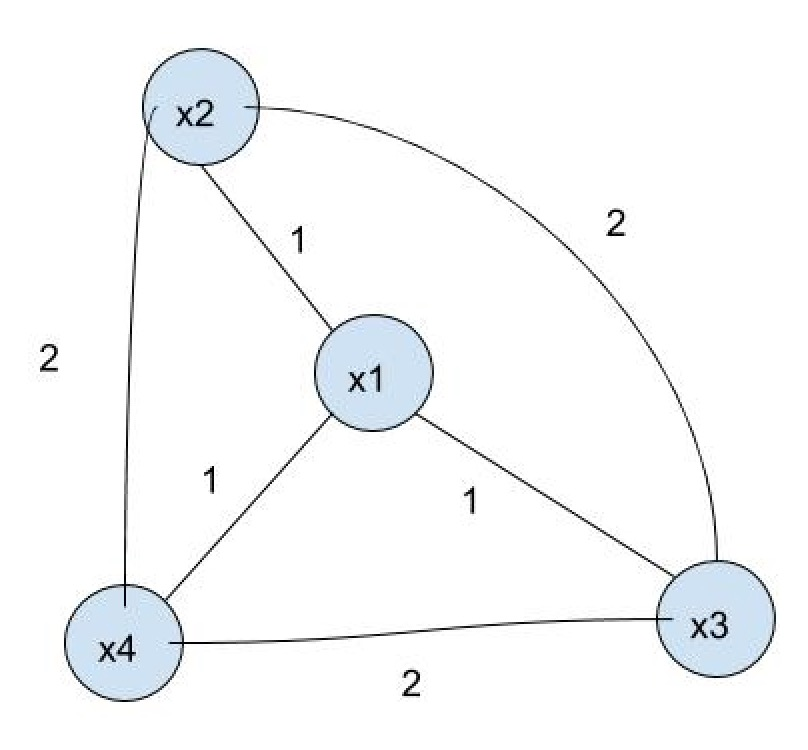
\includegraphics[width=0.5\textwidth]{chapter_5/files/unembeddable.jpg}
\caption{An illustration of a distance metric not embeddable in $l_2^d$ for any $d \in \bbN$.
We prove this by contradiction. Suppose we could embed $x_1, x_2, x_3, x_4$ into a Euclidean space isometrically.
According to the triangle inequality, $(x_1 ,x_2, x_3)$, $(x_1, x_2, x_3)$, $(x_1, x_3, x_4)$ are all collinear.
Thus, $x_1, x_2, x_3, x_4$ are collinear with each other.
However, no matter how we arrange the 4 points in a line,
we cannot make the distance between one point and other three points equal.
Thus there is no isometric embedding of these points into Euclidean space.}
\label{fig:unembeddable}
\end{center}
\end{figure}

\begin{definition}
Given two metric space $(X,\rho), (Y,\sigma)$. A mapping $f:
X\rightarrow Y$ is said to be a \emph{$D$-embedding} of $X$ into $Y$
(for $D\geq 1$) if there exists some $r>0$ such that $\forall x,x'
\in X$, 
\[
r \cdot \rho(x,x') \leq \sigma(f(x),f(x')) \leq D \cdot r \cdot
\rho(x,x').
\]
$D$ is said to be the \emph{distortion} of the embedding $f$, and if $D=1$, $f$ is isometric.
\end{definition}
